\documentclass[answers]{exam}
\usepackage{../../mypackages}
\usepackage{../../macros}


\SolutionEmphasis{\color{blue}}
\renewcommand{\solutiontitle}{\noindent}


\title{DST N°4 - Dérivées et analyses de fonctions}
\author{N. Bancel}
\date{26 Mars 2025}

\begin{document}

\textbf{Collège Lycée Suger}
\hfill
\textbf{Mathématiques} \\

\textbf{Année 2024-2025 - 3ème trimestre}
\hfill
\textbf{1ères STD2A} \par

{\let\newpage\relax\maketitle}

\begin{center}
\textbf{\textcolor{red}{Durée : 2 heures. La calculatrice n'est pas autorisée}} \\
\textbf{\textcolor{red}{Une réponse donnée sans justification sera considérée comme fausse.}} \\
Cette interrogation contient \numquestions\ questions, sur \numpages\ pages et est notée sur 20 points. 

\end{center}

\section*{Exercice 1 : Frise et pavage (2.5 points)}

\begin{questions} 

\question[1] Dans la frise ci-dessous :
\begin{compactitem}
  \item Repérer le motif
  \item Tracer le vecteur permettant de construire la frise à partir du motif
  \item Compléter la frise avec 2 motifs supplémentaires
\end{compactitem}

\begin{figure}[H]
  \centering
  \includegraphics[width=0.8\linewidth]{img/dst_04_01.jpg}
\end{figure}

\question[1.5] Dans la frise ci-dessous :
\begin{compactitem}
  \item Repérer la maille élémentaire et le motif
  \item Donner les transformations géométriques permettant de passer de la maille au motif
  \item Tracer le vecteur permettant de construire la frise à partir du motif
  \item Compléter la frise
\end{compactitem}

\begin{figure}[H]
  \centering
  \includegraphics[width=0.8\linewidth]{img/dst_04_02.jpg}
\end{figure}

\end{questions}

\section*{Exercice 2 : Analyse - Questions de cours (4 points)}

\begin{questions}

\question[2] Donner l'équation d'une droite, et nommer et définir les coefficients qui composent cette équation.
\begin{solution}
  L'équation d'une droite dans un repère est généralement donnée sous la forme :
  
  \[
  y = ax + b
  \]
  
  où :
  \begin{itemize}
    \item \( a \) est le \textbf{coefficient directeur} de la droite : il indique le \textit{sens de variation} (croissant si \( a > 0 \), décroissant si \( a < 0 \)) et la \textit{pente} de la droite.
    \item \( b \) est l'\textbf{ordonnée à l’origine} : c’est la valeur de \( y \) lorsque \( x = 0 \), autrement dit l’endroit où la droite coupe l’axe des ordonnées.
  \end{itemize}
  
  Par exemple, une droite d’équation \( y = 2x + 1 \) a un coefficient directeur \( a = 2 \) et une ordonnée à l’origine \( b = 1 \). Elle passe donc par le point \( (0 ; 1) \) et monte de 2 unités verticales à chaque unité horizontale.
  \end{solution}
\question[2] Reproduire le tableau ci-dessous sur sa copie et remplir la colonne 2 :

\vspace{0.5cm}

\begin{center}
\renewcommand{\arraystretch}{2} % augmente la hauteur des lignes
\begin{tabular}{|p{8cm}|p{6cm}|}
\hline
\textbf{Fonction $f$} & \textbf{Dérivée} \\
\hline
$f(x) = 6$ &  \\
\hline
$f(x) = x$ &  \\
\hline
$f(x) = x^2$ &  \\
\hline
$f(x) = x^3$ &  \\
\hline
\end{tabular}
\end{center}

\vspace{0.5cm}

\end{questions}

\begin{solution}
  
\vspace{0.5cm}

\begin{center}
\renewcommand{\arraystretch}{2}
\begin{tabular}{|p{8cm}|p{6cm}|}
\hline
\textbf{Fonction $f$} & \textbf{Dérivée} \\
\hline
$f(x) = 6$ & $f'(x) = 0$ \\
\hline
$f(x) = x$ & $f'(x) = 1$ \\
\hline
$f(x) = x^2$ & $f'(x) = 2x$ \\
\hline
$f(x) = x^3$ & $f'(x) = 3x^2$ \\
\hline
\end{tabular}
\end{center}
\end{solution}

\section*{Exercice 3 : Équations de droites (6 points)}

\begin{questions}

\question[2] Donner l’équation de la droite représentée ci-dessous.

\begin{figure}[H]
  \centering
  \includegraphics[width=0.5\linewidth]{img/dst_04_03.jpg}
\end{figure}


\begin{solution}
  On repère deux points appartenant à la droite et dont les coordonnées sont facilement lisibles car ce sont des nombres entiers :
  
  \[
  A(0 ; 1) \quad \text{et} \quad B(-2 ; 5)
  \]
  
  On peut alors calculer le **coefficient directeur** \( a \) de la droite à l’aide de la formule :
  \[
  a = \frac{y_B - y_A}{x_B - x_A} = \frac{5 - 1}{-2 - 0} = \frac{4}{-2} = -2
  \]
  
  Puisque la droite passe par le point \( A(0 ; 1) \), on en déduit que l’ordonnée à l’origine est :
  \[
  b = 1
  \]
  
  L’équation de la droite est donc :
  \[
  y = -2x + 1
  \]
  
  \vspace{0.3cm}
  \textbf{Conclusion :} Il y a deux choses que l’on peut vérifier assez facilement sur le graphique :
  \begin{itemize}
    \item Le signe du coefficient directeur est **négatif** (\( a = -2 \)), ce qui indique que la droite est \textbf{décroissante}. On observe bien sur le graphique que la courbe descend de la gauche vers la droite.
    \item L’\textbf{ordonnée à l’origine} est bien \( 1 \), ce qui est cohérent avec notre choix du point \( A(0 ; 1) \). On voit que la droite coupe l’axe des ordonnées en \( y = 1 \).
  \end{itemize}
  \end{solution}

\question[4] Équation de droite :

\begin{parts}
  \part[2] Tracer la droite d’équation $f(x) = 3x - 2$
  \begin{solution}
    Pour tracer une droite, il suffit de repérer deux points appartenant à cette droite, puis de les relier à la règle.
    
    On peut choisir deux valeurs simples pour \( x \), par exemple :
    \[
    \begin{cases}
    x = 0 \Rightarrow f(0) = 3 \times 0 - 2 = -2 \Rightarrow (0 ; -2) \\
    x = 1 \Rightarrow f(1) = 3 \times 1 - 2 = 1 \Rightarrow (1 ; 1)
    \end{cases}
    \]
    
    On place donc les points \( A(0 ; -2) \) et \( B(1 ; 1) \) sur le repère, puis on trace la droite qui passe par ces deux points.
    
    \begin{figure}[H]
      \centering
      \includegraphics[width=0.5\linewidth]{img/dst_04_04.jpg}
    \end{figure}
    

    \textit{Astuce : on peut choisir n’importe quelles valeurs de \( x \), mais il est préférable de choisir des valeurs simples pour lesquelles le calcul de \( f(x) \) donne un entier. Cela facilite le tracé.}
    \end{solution}


  \part[0.5] Comment pouvait-on deviner son sens de variation ?

  \begin{solution}
    La fonction \( f(x) = 3x - 2 \) est une fonction affine de coefficient directeur \( a = 3 \). Ce coefficient est \textbf{strictement positif}, donc on sait que :
    
    \[
    f \text{ est strictement croissante sur } \mathbb{R}
    \]
    
    Graphiquement, cela signifie que la droite monte de la gauche vers la droite.
    \end{solution}
  \part[1.5] Dresser le tableau de signes de $f$ entre $-\infty$ et $+\infty$ :

\begin{solution}
  On cherche pour quelles valeurs de \( x \) la fonction s’annule :
  \[
  f(x) = 3x - 2 = 0 \Rightarrow x = \frac{2}{3}
  \]
  
  On établit ensuite le tableau de signes de \( f(x) \) :
  
  \begin{center}
  \begin{tikzpicture}
    \tkzTabInit{$x$ / 1 , $f(x)$ / 1}{$-\infty$, $\dfrac{2}{3}$, $+\infty$}
    \tkzTabLine{ , -, z, + , }
  \end{tikzpicture}
  \end{center}
  
  Ainsi :
  \begin{itemize}
    \item \( f(x) < 0 \) pour \( x < \dfrac{2}{3} \)
    \item \( f(x) = 0 \) pour \( x = \dfrac{2}{3} \)
    \item \( f(x) > 0 \) pour \( x > \dfrac{2}{3} \)
  \end{itemize}
  \end{solution}
\end{parts}

\end{questions}

\section*{Exercice 4 : Étude des variations d’un polynôme (7.5 points)}

\begin{questions}

\question[1.5] Soit la fonction $f(x) = x^2 + 2x - 3$. Calculer l’expression de la dérivée de $f$.
\begin{solution}
  La dérivée de $f$ est :
  \[ f'(x) = 2x + 2 \]
  \end{solution}

\question[1.5] Étudier le signe de la dérivée de $f$ (on pourra dresser un tableau de signes).

\begin{solution}
  On cherche à déterminer la valeur de $x$ pour laquelle $f'$ s'annule. Ce qui revient à résoudre l'équation : \\
  \[
  f'(x) = 2x + 2 = 0 \Rightarrow x = -1
  \]
  $f'$ a la forme d'une fonction affine avec $a=2$ et $b=2$. \\
  $a$ est donc de signe positif et par application du cours on peut conclure que \\

  \[
  \begin{cases}
    \forall x < -1 \text{,} f'(x) < 0 \\
    \forall x > -1 \text{,} f'(x) > 0
  \end{cases}
\]

\begin{tikzpicture}
  \tkzTabInit{$x$ / 1 , $f'(x)$ / 1}{$-\infty$, -1, $+\infty$}
  \tkzTabLine{, -, z, +, }
\end{tikzpicture}

\end{solution}

\question[1] En déduire le sens de variation de la fonction $f$ (prendre soin de citer les propriétés qui permettent de déduire le sens de variation).

\begin{solution}
  On sait que la dérivée d'une fonction donne des indications sur son sens de variation :
  
  \begin{itemize}
    \item Si $f'(x) > 0$ sur un intervalle, alors $f$ est croissante sur cet intervalle.
    \item Si $f'(x) < 0$ sur un intervalle, alors $f$ est décroissante sur cet intervalle.
    \item Si $f'(x) = 0$ en un point isolé, cela peut correspondre à un extremum (maximum ou minimum).
  \end{itemize}

D'après la question précédente, on peut déduire les variations de $f$ :

\begin{itemize}
  \item Sur $]-\infty, -1[$, $f'(x) < 0$ donc $f$ est décroissante.
  \item Sur $]-1, +\infty[$, $f'(x) > 0$ donc $f$ est croissante.
  \item En $x = -1$, la dérivée s’annule, donc $f$ admet un minimum local en $x = -1$.
\end{itemize}

On peut donc dresser le tableau de variations de $f$ superposé à celui du signe de sa dérivée :

\begin{center}
\begin{tikzpicture}
  \tkzTabInit[lgt=2.5]
  {$x$ / 1 , $f'(x)$ / 1 , $f(x)$ / 2}{$-\infty$, $-1$, $+\infty$}
  \tkzTabLine{, -, z, +, }
  \tkzTabVar{+/ , -/$f(-1)$ , +/ }
\end{tikzpicture}
\end{center}

Pour finir, on calcule la valeur exacte de $f(-1)$ :
\[
f(-1) = (-1)^2 + 2(-1) - 3 = 1 - 2 - 3 = -4
\]

Et on peut préciser le tableau :

\begin{center}
\begin{tikzpicture}
  \tkzTabInit[lgt=2.5]
  {$x$ / 1 , $f'(x)$ / 1 , $f(x)$ / 2}{$-\infty$, $-1$, $+\infty$}
  \tkzTabLine{, -, z, +, }
  \tkzTabVar{+/ , -/$-4$ , +/ }
\end{tikzpicture}
\end{center}
\end{solution}

\question[1] Déterminer le taux d’accroissement de la fonction $f$ entre $-1$ et $2$.
\begin{solution}
  Le **taux d'accroissement** de la fonction $f$ entre $x = -1$ et $x = 2$ est donné par la formule :
  
  \[
  \frac{f(2) - f(-1)}{2 - (-1)} = \frac{f(2) - f(-1)}{3}
  \]
  
  Calculons les valeurs de $f$ en $-1$ et en $2$ :
  
  \[
  f(-1) = (-1)^2 + 2 \times (-1) - 3 = 1 - 2 - 3 = -4
  \]
  
  \[
  f(2) = (2)^2 + 2 \times 2 - 3 = 4 + 4 - 3 = 5
  \]
  
  On en déduit le taux d'accroissement :
  
  \[
  \frac{f(2) - f(-1)}{3} = \frac{5 - (-4)}{3} = \frac{9}{3} = 3
  \]
  
  \textbf{Conclusion :} Le taux d'accroissement de $f$ entre $-1$ et $2$ est égal à $3$.
  \end{solution}
\question[1.5] Tracer la courbe représentative de $f$.

\question[1] Quelle est l’interprétation graphique du taux de variation calculé à la question précédente ? Cette interprétation est-elle bien vérifiée sur la figure tracée ?
\begin{solution}
  Le taux d'accroissement entre $x = -1$ et $x = 2$ correspond au **coefficient directeur de la droite sécante** passant par les points $A(-1, f(-1))$ et $B(2, f(2))$.
  
  Dans notre cas :
  \[
  f(-1) = -4 \quad \text{et} \quad f(2) = 5
  \]
  
  La droite sécante passe donc par les points $A(-1, -4)$ et $B(2, 5)$, et son coefficient directeur est :
  \[
  \frac{f(2) - f(-1)}{2 - (-1)} = 3
  \]
  
  \textbf{Interprétation graphique} :  
  On peut dire que la courbe $f$ monte en moyenne de 3 sur l'axe des ordonnées quand on avance de 1 sur l'axe des abscisses. 
  
  \textbf{Vérification graphique} :   
  xxxx
  
  \end{solution}
\end{questions}


\end{document}
